%%\documentclass[t]{beamer}   % overlays
\documentclass[t,handout]{beamer}   % no overlays
%%\setbeameroption{show notes}     % create slides with notes

\usetheme{Madrid}
\usecolortheme{beaver}
\usepackage{tikz}
\usetikzlibrary{fit,arrows,calc,positioning}

%\usepackage{emerald} 
\usepackage[T1]{fontenc} 


\usepackage{graphicx}
\usepackage{epsfig}
\usepackage{psfrag}
\usepackage[english]{babel}
\usepackage{listings}
\usepackage{courier}
\usepackage{color}
\usepackage[backend=bibtex,style=ieee]{biblatex}

\lstset{
	language=Ruby,
	basicstyle=\footnotesize\ttfamily\color{black},
	commentstyle = \footnotesize\ttfamily\color{red},
	keywordstyle=\footnotesize\ttfamily\color{blue},
	stringstyle=\footnotesize\ttfamily\color{black},
%	columns=fixed,
%	numbers=left,    
	numberstyle=\tiny,
	stepnumber=1,
	numbersep=5pt,
	tabsize=1,
	extendedchars=true,
	breaklines=true,            
	frame=b,         
	showspaces=false,
	showtabs=true,
	xleftmargin=6pt,
	framexleftmargin=6pt,
	framexrightmargin=2pt,
	framexbottommargin=4pt,
	showstringspaces=false      
}

\lstloadlanguages{
         Ruby,HTML
}

\graphicspath{ {./images/} }  % Figures path - used in graphicx

%\selectcolormodel{cmyk}

\mode<presentation>

\renewcommand*{\bibfont}{\tiny}

\newcommand{\dred}{darkred!90!black}
\newcommand{\written}{\ECFJD\textcolor{cyan!50!white}}
\newcommand{\hlight}{\textcolor{\dred}}
\newcommand{\Ex}{\textcolor{\dred}{Ex. }}

% remove navigation symbols in full screen mode
\setbeamertemplate{navigation symbols}{}  
\setbeamertemplate{blocks}[rounded][shadow=false]
\setbeamertemplate{itemize items}[default]
\setbeamertemplate{enumerate items}[default]
\setbeamertemplate{sections/subsections in toc}[circle]
\setbeamercolor{note page}{fg=black}

\setbeamercolor{title}{fg=\dred}
\setbeamercolor{frametitle}{fg=white}
\setbeamercolor{frametitle}{bg=\dred}
\setbeamercolor{structure}{fg=black,bg=white}
\setbeamercolor{background canvas}{bg=white,fg=black}
\setbeamercolor{normal text}{fg=black,bg=white}
\setbeamercolor{item}{fg=red!80!black,bg=white!}
\addtobeamertemplate{block begin}{\setbeamercolor{block title}{fg=white,bg=\dred}
\setbeamercolor{block body}{fg=\dyellow,bg=gray!50!black}}{}



\addbibresource{bib/aws.bib}

\title[Cohort Analytics]
{Cohort Analytics and Cloud Usage: Security Review}

\author[Heileman, Babbitt \& Abdallah] % (optional, use only with lots of authors)
{\bf Greg Heileman \ \ \ \ \ Terry Babbitt \ \ \ \ \ Chaouki Abdallah}

\institute[UNM]
{Application Development Team \\
Academic Affairs \\
University of New Mexico}

\date[June 26, 2015]

\begin{document}

\begin{frame}
  \titlepage
\end{frame}
\note{Talk for 10 minutes} 

\addtobeamertemplate{frametitle}{}{%
\begin{tikzpicture}[remember picture,overlay]
\node[anchor=north east,yshift=-1pt] at (current page.north east) {
\includegraphics[width = 1in]{UNMLogo.png}};
\end{tikzpicture}}

%%%%%%%%%%%%%%%%%%%%%%%%%%%%%%%%%%%%%%%%%%%%%%%%%%%%%%

%\section*{Outline}
%
%\begin{frame}  \frametitle{Outline}  
%	\tableofcontents
%\end{frame}

\section{Introduction}

\begin{frame}{Cohort Analytics -- Overview}%%%%%%%%%%%%%%%%%%%%%%%%%%%%%%%%%%%%

\vspace*{-0.2in}
\textbf{We have developed a cohort analytics application that will dramatically improve our student success capabilities.}~\\~\\
\pause
This application will enable:
\begin{itemize}
\item Advisors, chairs, deans and administrators to track the progress of relevant student cohorts relative to academic progress. 
\pause
\item Earlier insights into various metrics the regents, president, provost have asked us to track.  E.g., accurately project the number of students who will graduate in four years (tuition free final semester).
\pause
\item The ability to set and track program- and college-level success targets.
\pause
\item More accurate graduation rate projections (years in advance, rather than months in advance of required reporting). 
\end{itemize}~\\
\pause
{\bf Target Date for Release: August 7, 2015}
\end{frame}

\begin{frame}{Cohort Analytics Dashboard}%%%%%%%%%%%%%%%%%%%%%%%%%%%%%%%%%%%%
 \vspace*{-0.25in}
  \centerline{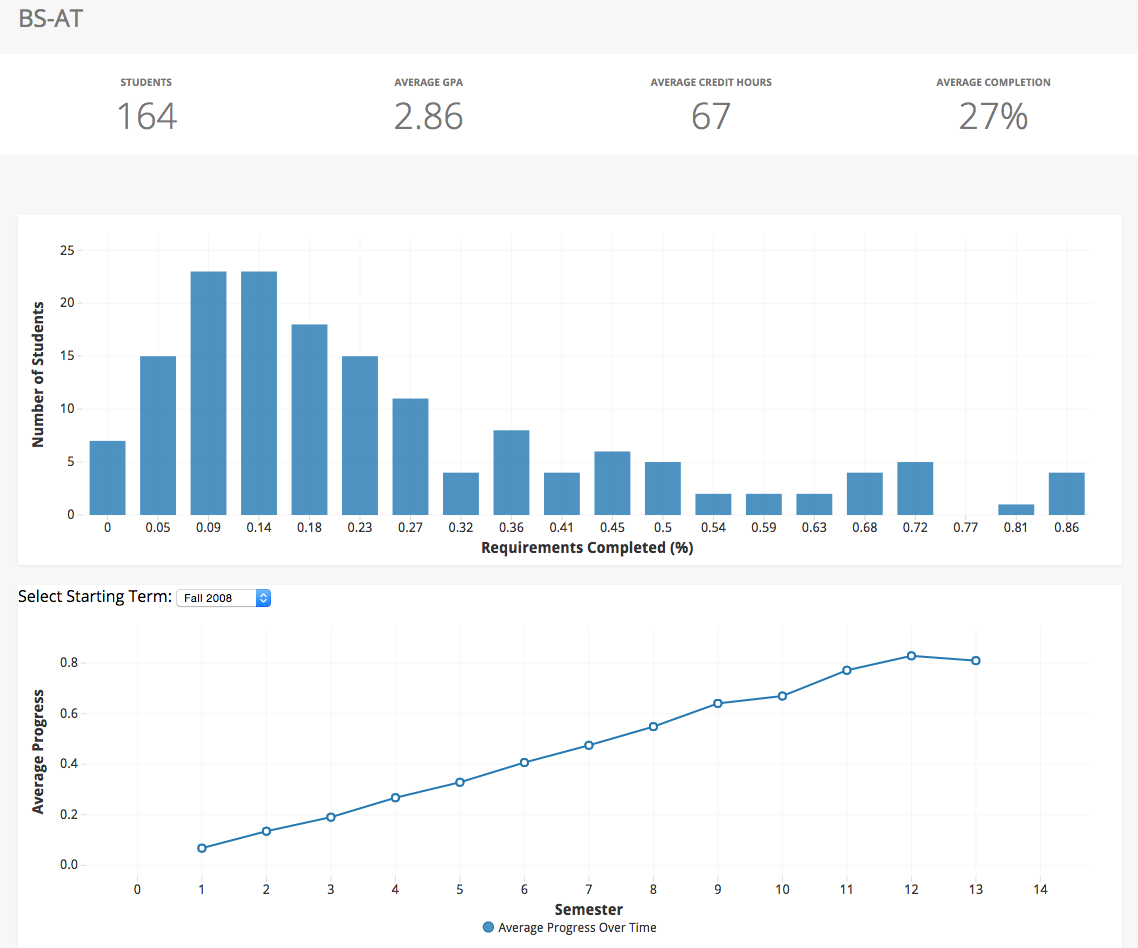
\includegraphics[width=3.75in]{Dashboard1.png}}
\end{frame}

\begin{frame}{Cohort Analytics Dashboard}%%%%%%%%%%%%%%%%%%%%%%%%%%%%%%%%%%%%
  \vspace*{-0.25in}
  \centerline{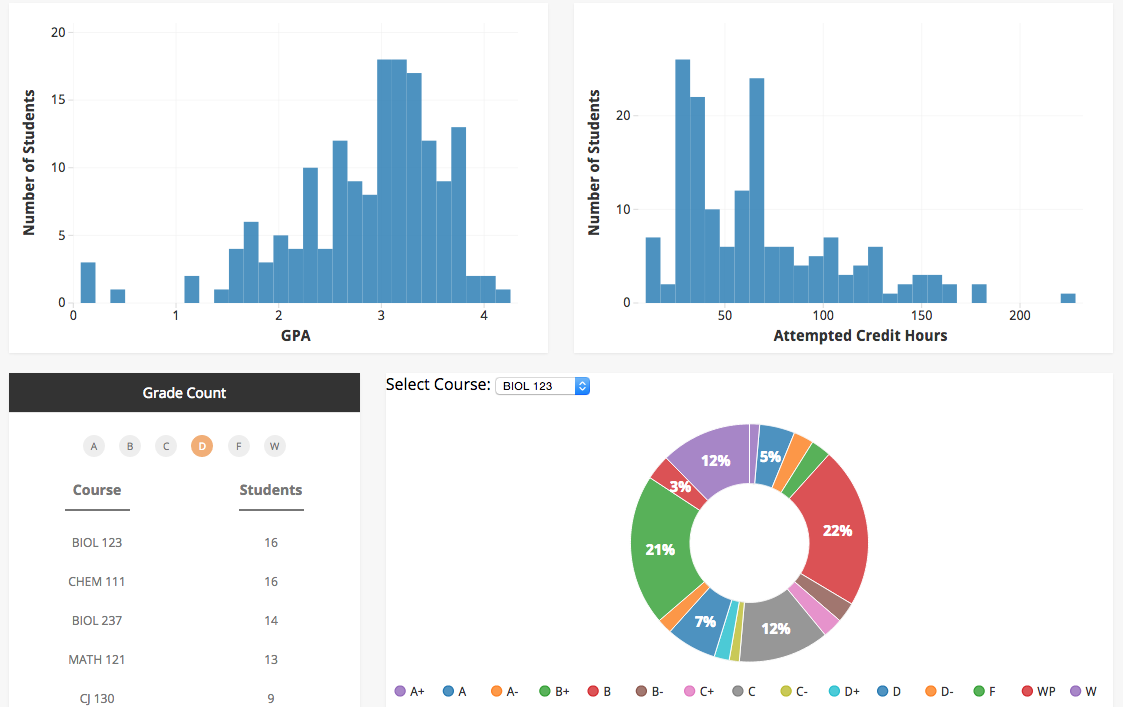
\includegraphics[width=4.75in]{Dashboard2.png}}
\end{frame}

\begin{frame}{Cohort Analytics Dashboard (fake names)}%%%%%%%%%%%%%%%%%%%%%%%%%%%%%%%%%%%%
 \vspace*{-0.25in}
  \centerline{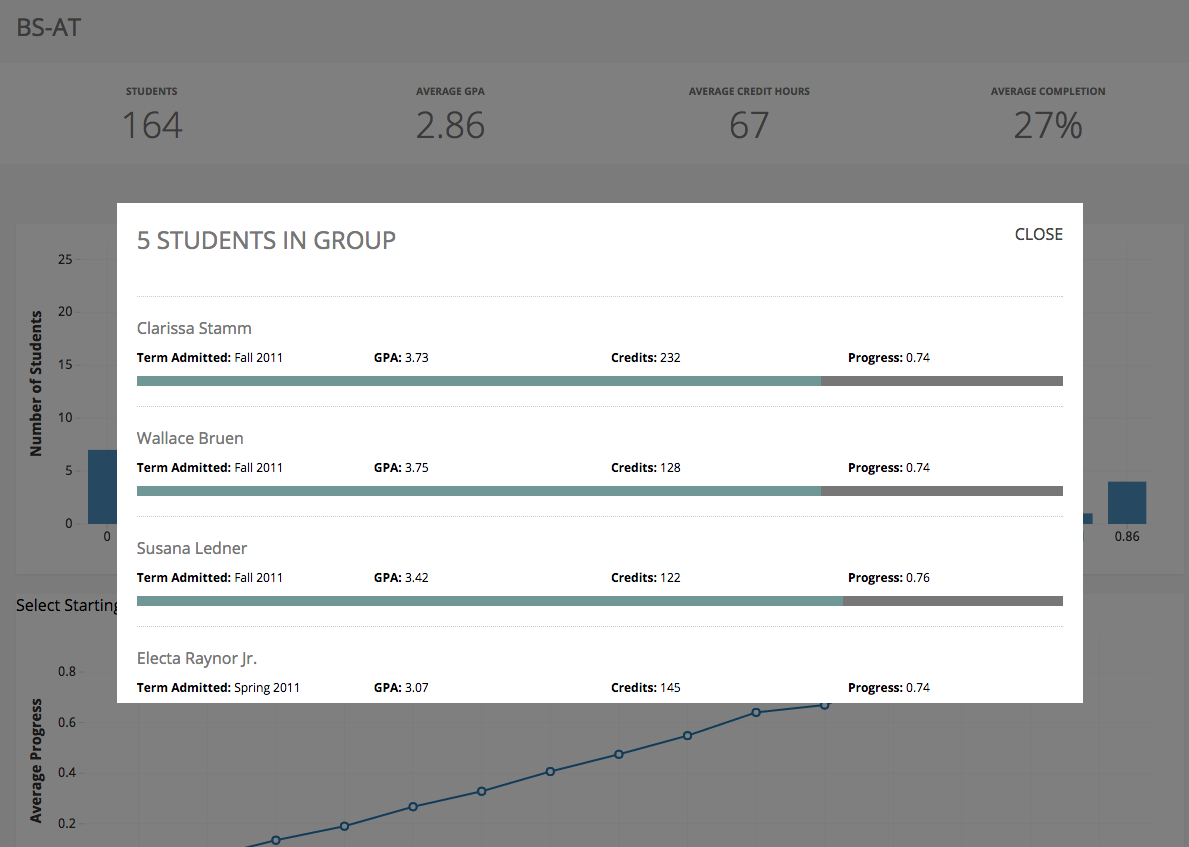
\includegraphics[width=4.35in]{Dashboard3.png}}
\end{frame}

\begin{frame}{Cohort Analytics Dashboard (fake name)}%%%%%%%%%%%%%%%%%%%%%%%%%%%%%%%%%%%%
  \vspace*{-0.25in}
  \centerline{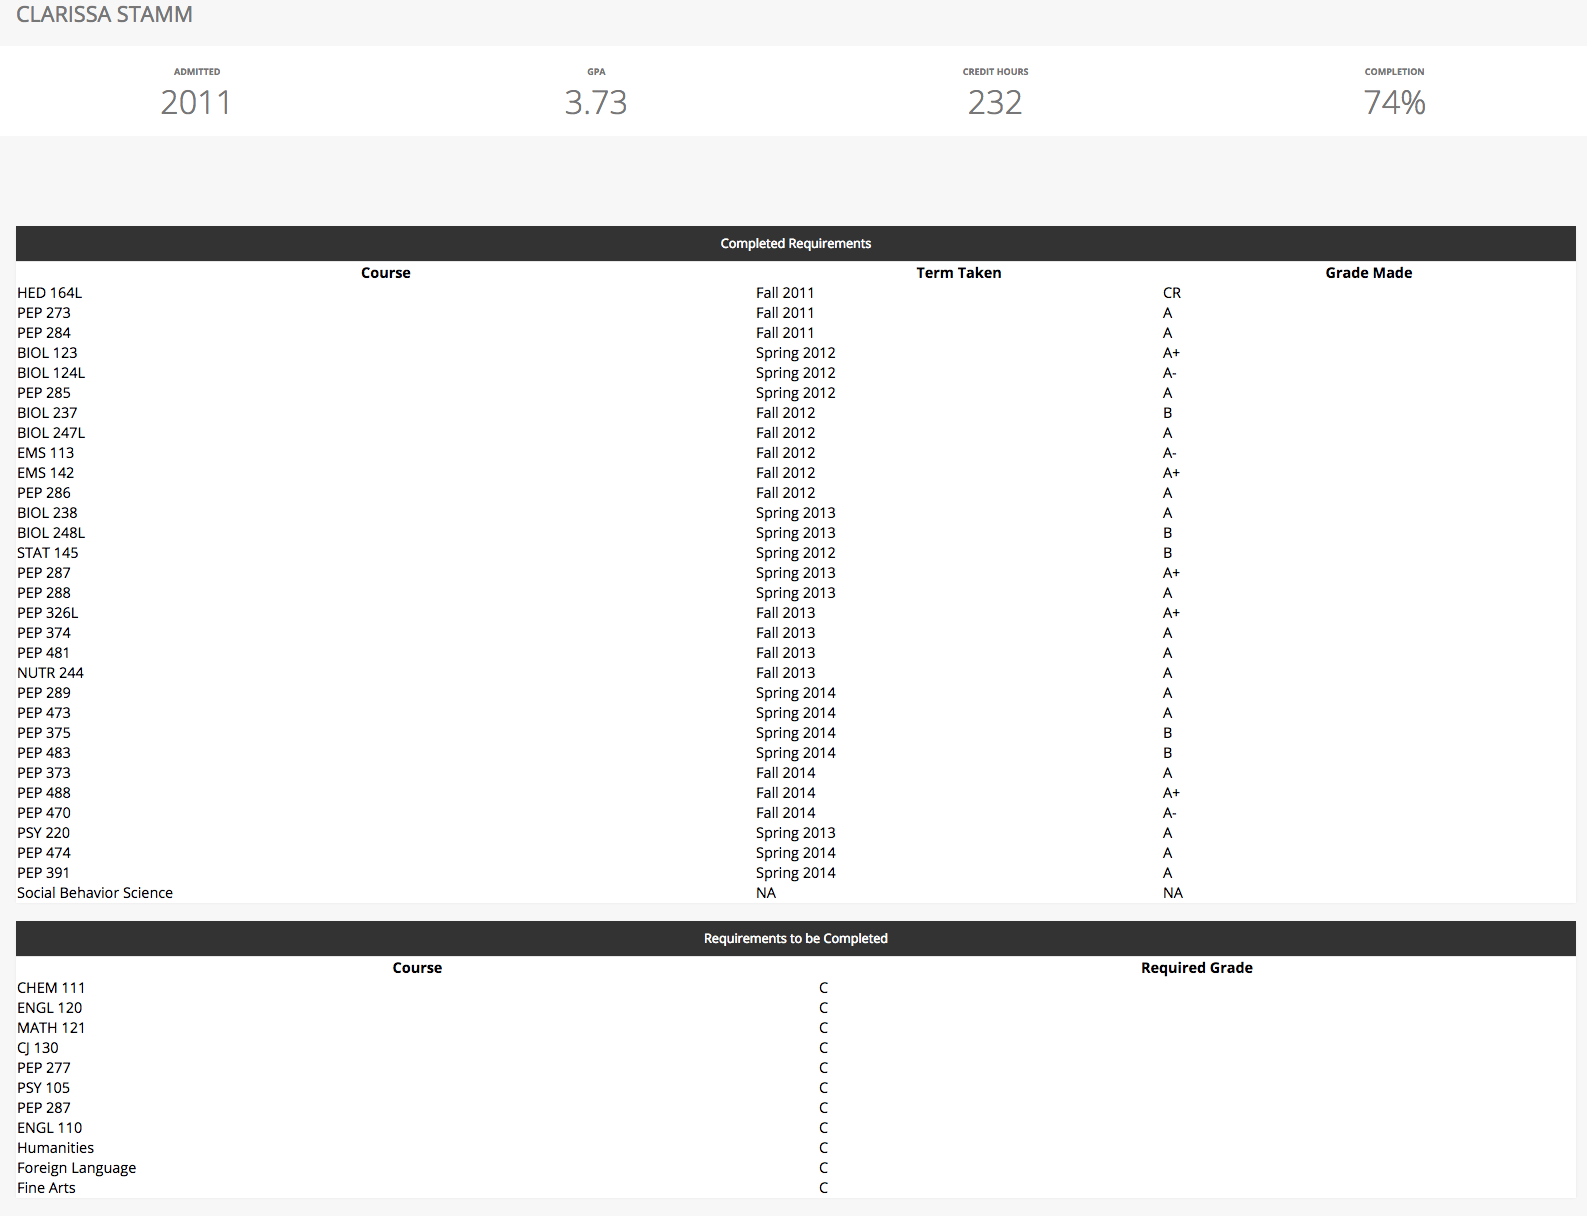
\includegraphics[width=4.2in]{Dashboard4.png}}
\end{frame}


\begin{frame}{Cohort Analytics -- Components}%%%%%%%%%%%%%%%%%%%%%%%%%%%%%%%%%%%%
The application involves the integration of a number of information systems:
\begin{itemize}
 \item Student Data Mart -- student progress data (FERPA applies).
 \pause
 \item Degree Requirements and Degree Plans databases.
 \pause 
 \item Reasoning Engine -- reasons over the aforementioned data stores.
 \pause
 \item CAS Authentication and Authorization (whitelist until BAR roles are made available).
 \pause
 \item Analytics and Interactive Dashboard Framework.
\end{itemize}~\\
\pause
{\bf Note: the system involves moving student data to Amazon Web Services.}
\end{frame}

\begin{frame}{Security Profile \& Controls~\footfullcite{UNM_ITS:08}}%%%%%%%%%%%%%%%%%%%%%%%%%%%%%%%%%%%%
\vspace*{-0.25in}
\textbf{UNM Data Classification:}
\begin{enumerate}
\item Data owners: students
\pause
\item Data steward: Enrollment Management (Terry Babbitt), Custodians: AA Application Development Team and end users
\pause
\item Information system identification: see slide~10
\pause
\item Data categorization: student data -- academic performance and other student attributes (e.g., ethnicity, gender, HS attended, etc.)
\pause
\item Privacy requirements: FERPA 
\pause
\item Data Classification: see next slide
\pause
\item UNM Information Security Safeguards guidance: not available (see attached document and the following slides for our security control selection analysis)
\end{enumerate}
\end{frame}

\begin{frame}{UNM Data Classification Worksheet~\footfullcite{UNM_ITS:08}}%%%%%%%%%%%%%%%%%%%%%%%%%%%%%%%%%%%%
\vspace*{-0.2in}
\textbf{Data Owner:} students~\\
\pause
\vspace*{0.1in}
\textbf{Information System (application name):} Cohort Analytics~\\
\pause
\vspace*{0.1in}
\textbf{Specific Pieces of Data:} student data -- academic performance and other student attributes (e.g., ethnicity, gender, HS attended, etc.)~\\
\pause
\vspace*{0.1in}
\textbf{Data Classification:} FIPS SC for cohort analytics data = \{(Confidentiality, Moderate), (Integrity, Low), ( Availability, Low)\}~\\  
\pause
\textbf{Note:} Moderate confidentiality requirements will be supported through controls including encryption at rest and in transit, via encryption standards described below. ~\\
\pause
\vspace*{0.1in}
\textbf{Rationale:} see attached document.~\\
\pause
\vspace*{0.1in}
The combination of the above data classification, and the appropriate controls given this classification, seem to imply UNM's ``C Class.''
\note[\item]{CONFIDENTIALITY
?Preserving authorized restrictions on information access and disclosure, including means for protecting personal privacy and proprietary information...? [44 U.S.C., Sec. 3542]~\\
A loss of confidentiality is the unauthorized disclosure of information. ~\\
INTEGRITY
?Guarding against improper information modification or destruction, and includes ensuring information non-repudiation and authenticity...? [44 U.S.C., Sec. 3542]~\\
A loss of integrity is the unauthorized modification or destruction of information.~\\
AV AILABILITY
?Ensuring timely and reliable access to and use of information...? [44 U.S.C., SEC. 3542]~\\
A loss of availability is the disruption of access to or use of information or an information system.}
\end{frame}

\section{Technical Components}%%%%%%%%%%%%%%%%%%%%%%%%%%%%%%%%%%%%
\begin{frame}{Cohort Analytics -- Technical Components}
\vspace*{0.25in}
  \centerline{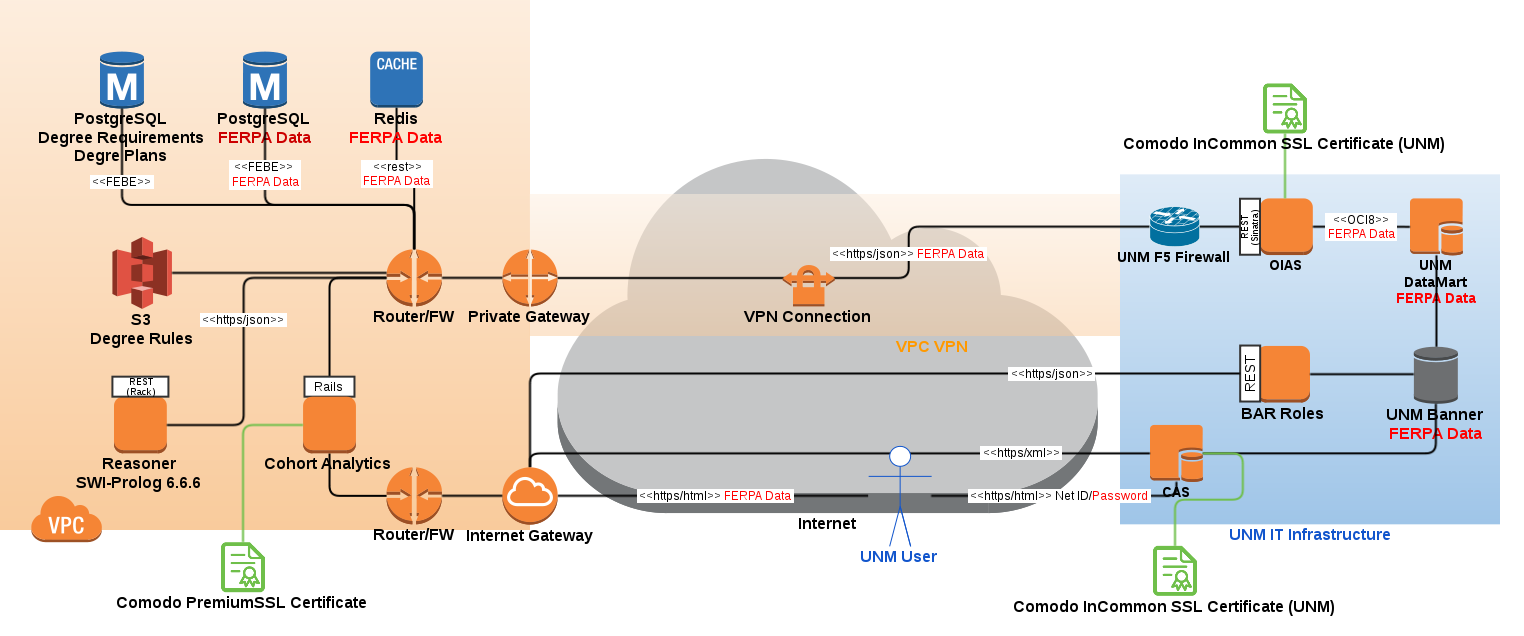
\includegraphics[width=4.9in,height=2.2in]{vpc_view_certs.png}}
\end{frame}

\section{Technical Components}%%%%%%%%%%%%%%%%%%%%%%%%%%%%%%%%%%%%
\begin{frame}{Cohort Analytics -- Technical Components}
\vspace*{-0.15in}
\textbf{Notes:}
\begin{itemize}
 \item Until the Banner Authorization Role (BAR) can be worked out, we will use UNM's CAS system for user authentication, and we will maintain a whitelist on the AWS side for user authorization. 
 \pause Whitelist entires must have UNM FERPA training, and if this is satisfied will include:
 \begin{itemize}
  \item UNM President and Provost Office administrators.
  \pause
  \item Deans, Chairs and Program-level administrators
  \pause
  \item Academic Advisors
  \pause
  \item Others with a justified business need.
 \end{itemize}~\\
  \pause
 \item For the required encrypted connections between these users and the Cohort Analytics system running on AWS, Academic Affairs will obtain a Premium SSL Certificate from Comodo.
\end{itemize}
\end{frame}


\section{Responsibilities}%%%%%%%%%%%%%%%%%%%%%%%%%%%%%%%%%%%%
\begin{frame}{Responsibilities - Infrastructure}
 	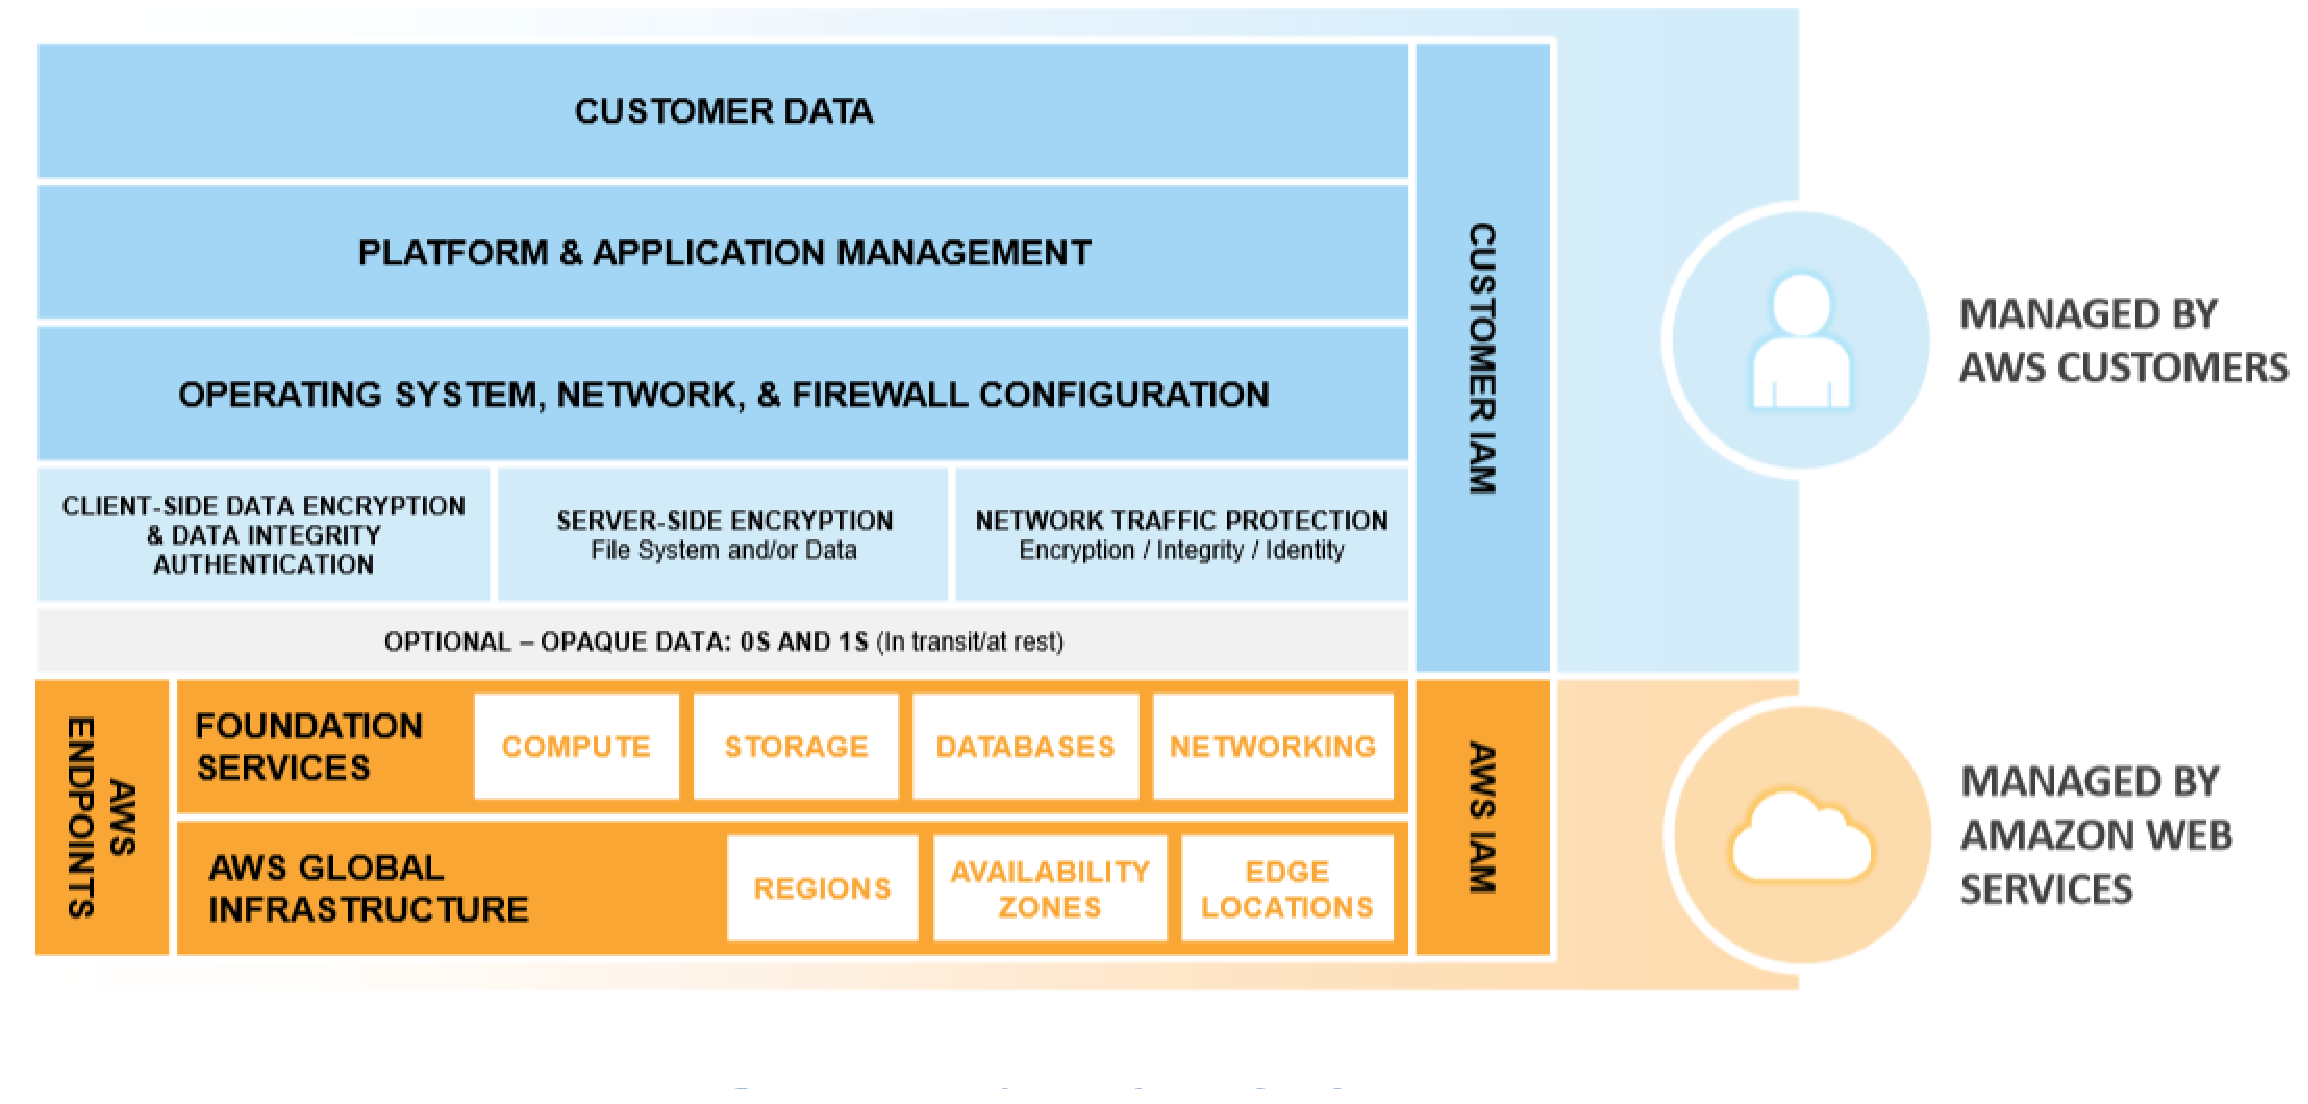
\includegraphics[width=\textwidth]{442-mod.pdf} \\
 	{\tiny Extracted from content provided by Amazon Web Services~\footfullcite{Aws:15}.}
\end{frame}

\begin{frame}{Responsibilities - Containers}%%%%%%%%%%%%%%%%%%%%%%%%%%%%%%%%%%%%
 	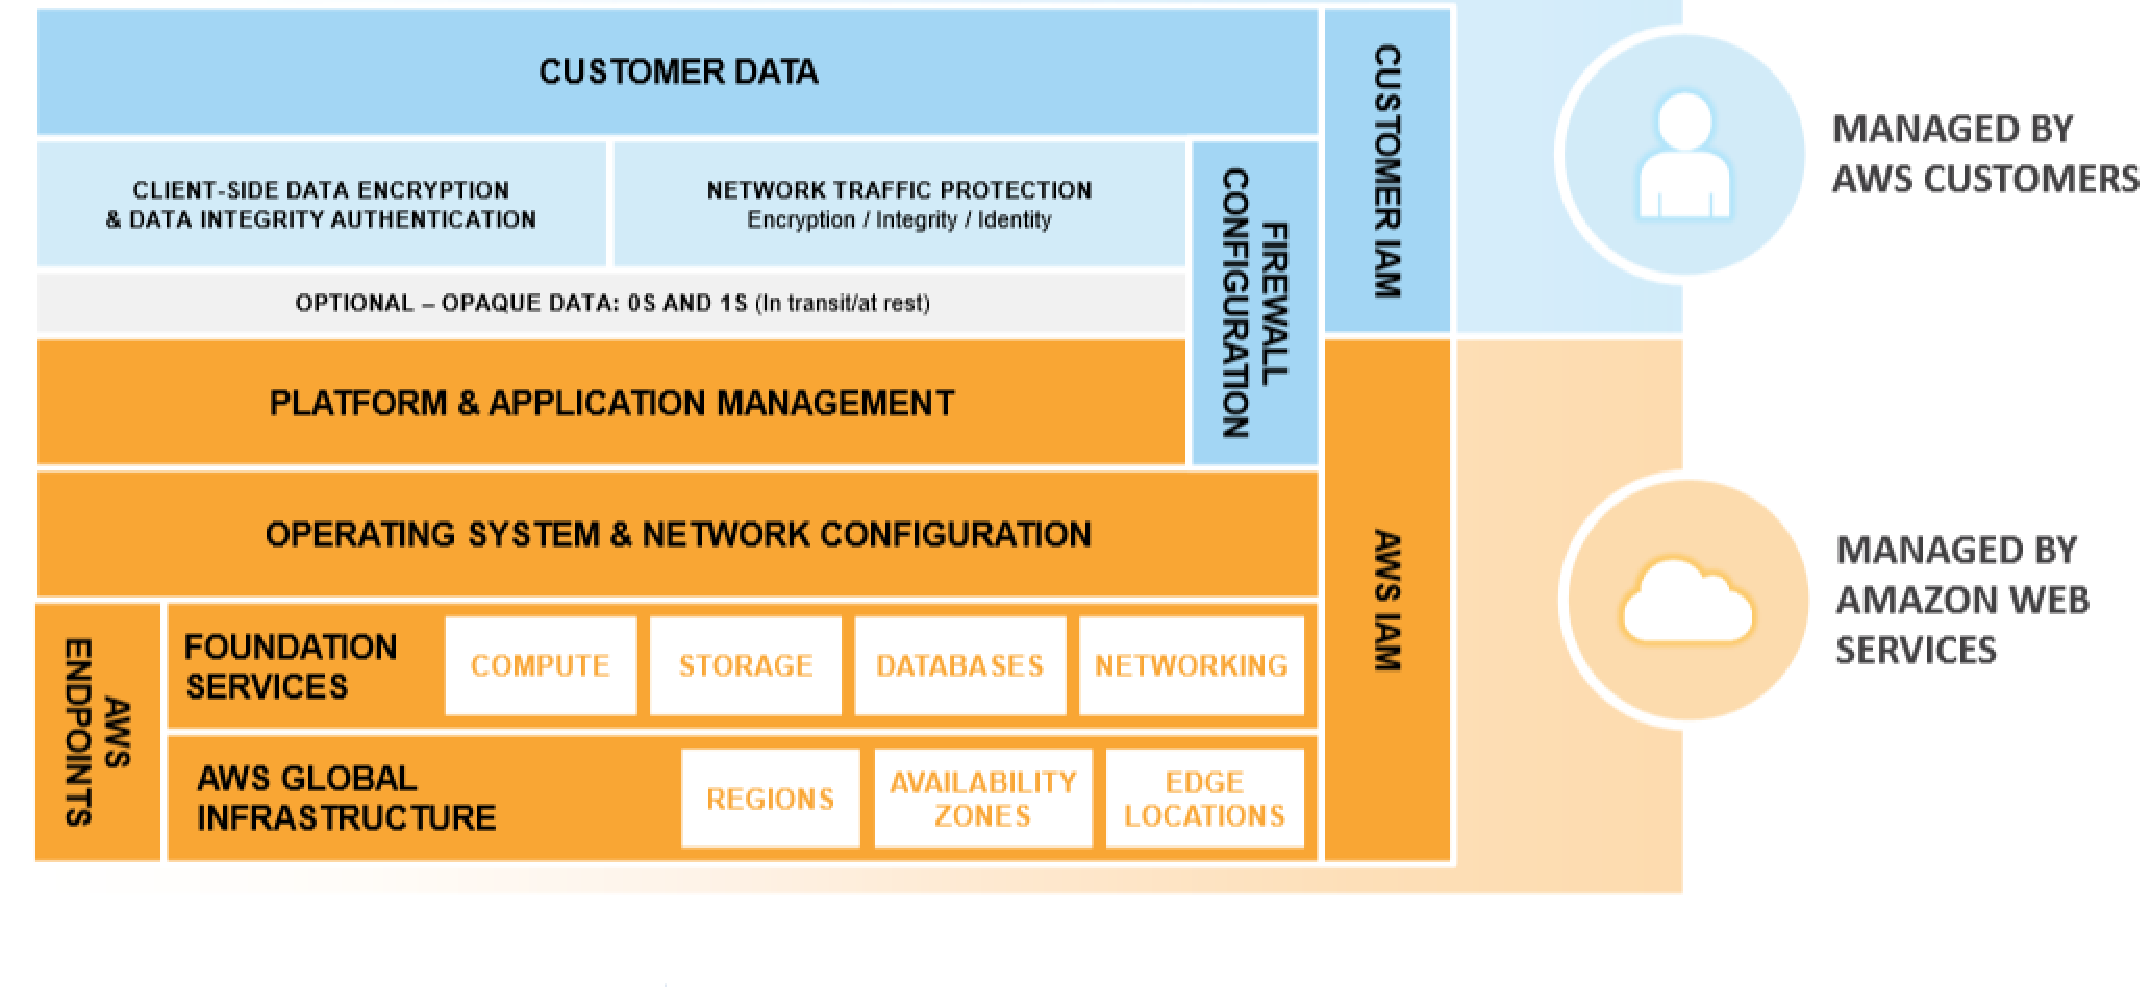
\includegraphics[width=\textwidth]{445-mod.pdf}
\end{frame}

\begin{frame}{Responsibilities - Abstract Services}%%%%%%%%%%%%%%%%%%%%%%%%%%%%%%%%%%%%
 	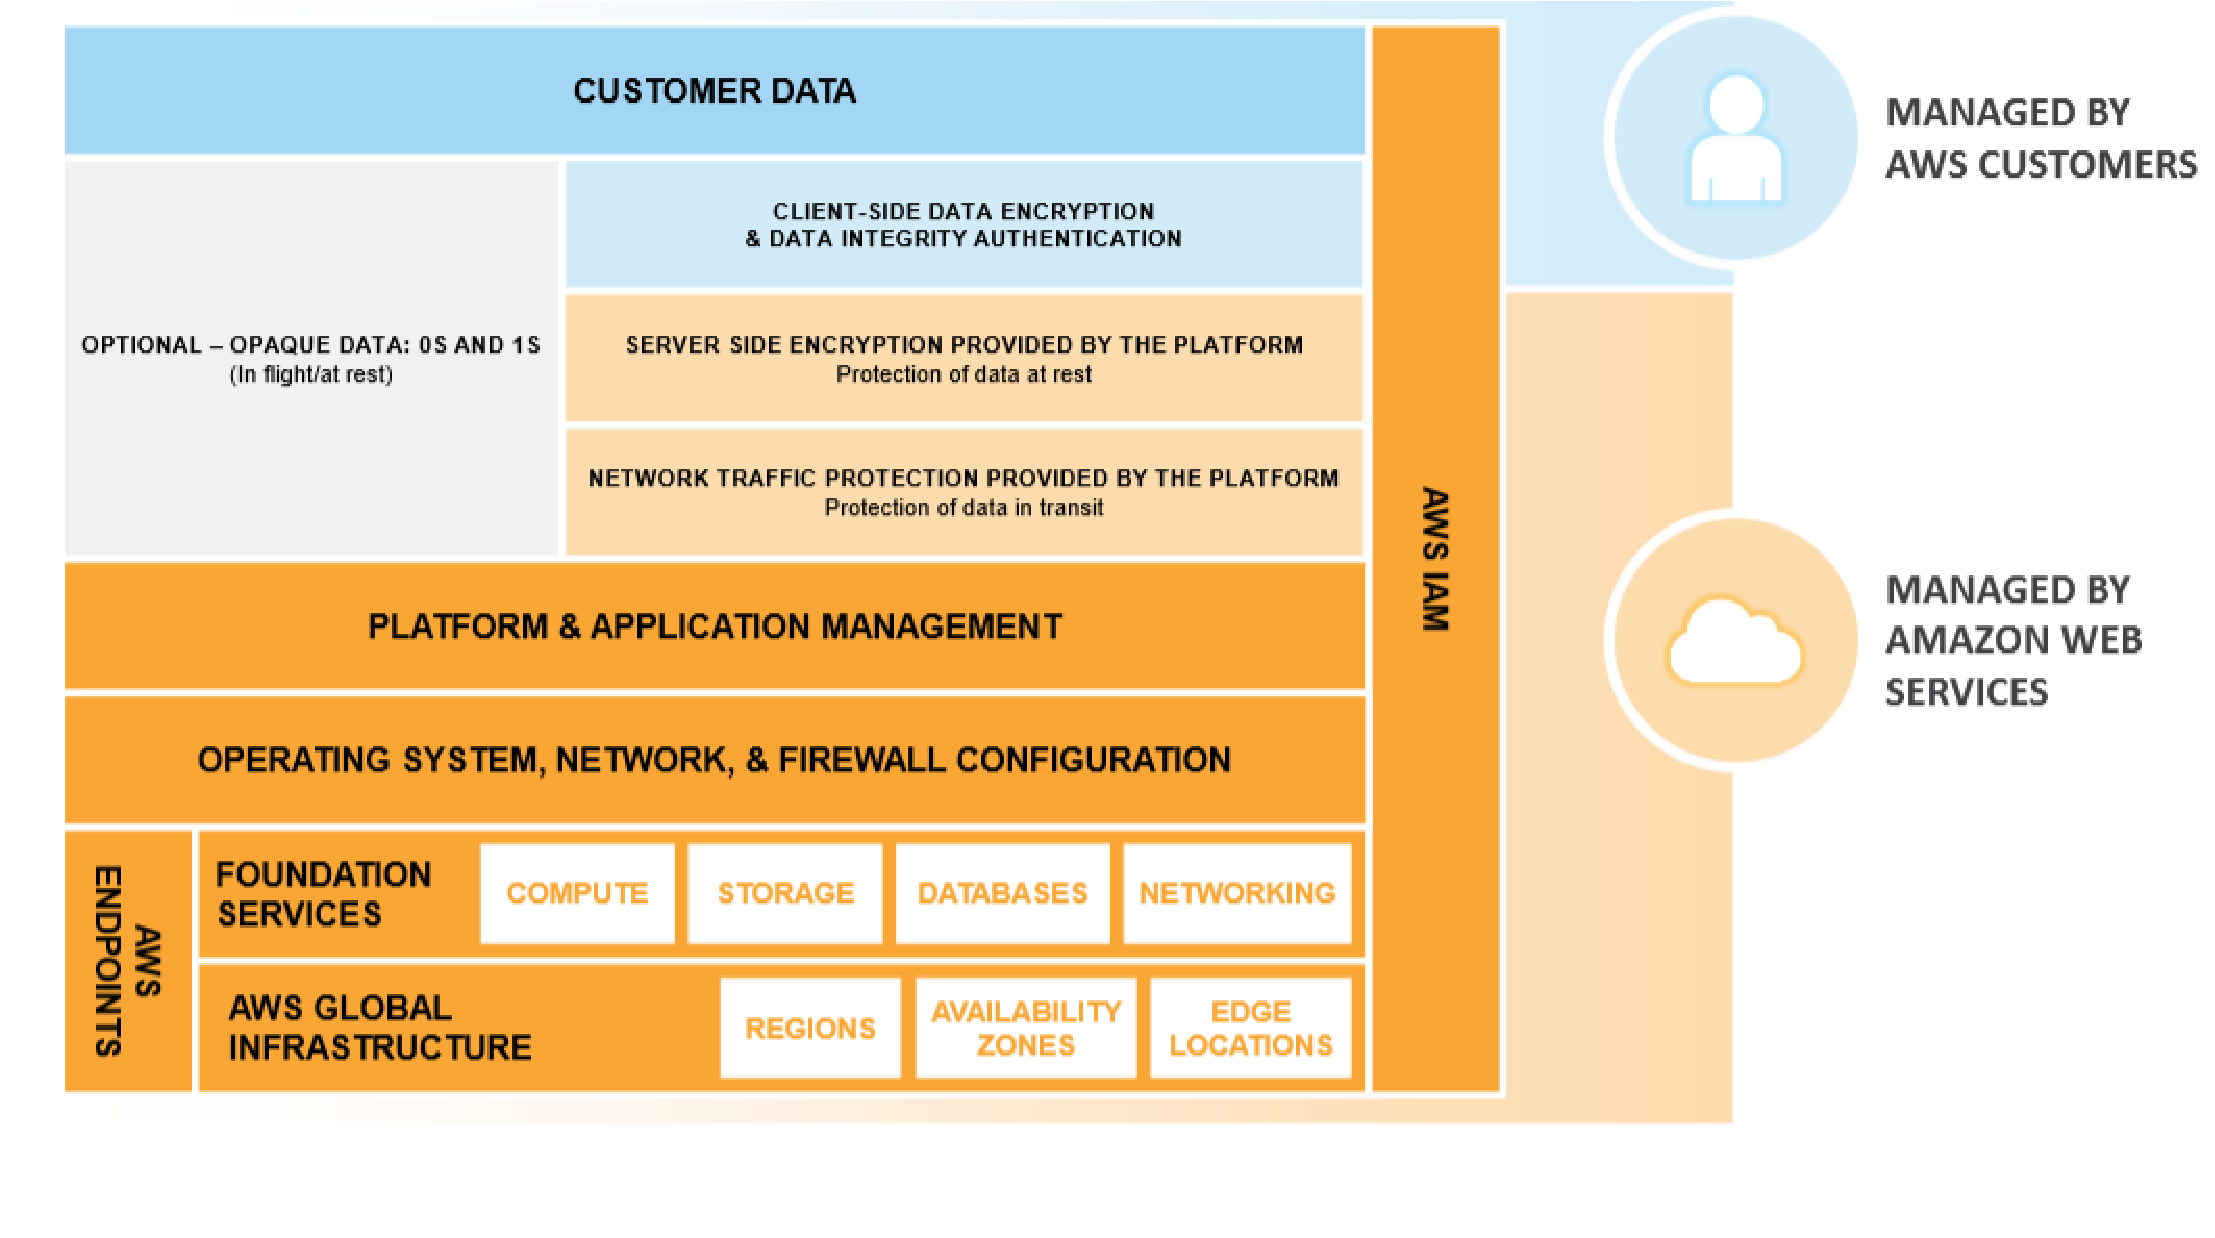
\includegraphics[width=\textwidth]{448-mod.pdf}
\end{frame}

\begin{frame}{Our Responsibilities - AWS}%%%%%%%%%%%%%%%%%%%%%%%%%%%%%%%%%%%%
\textbf{OS, Network, FW Configuration:}
{\small
\begin{itemize}
\item Elastic Compute Cloud (EC2) VMs run SELinux/Redhat, UFW
\item We don't manage UNM VMs or Firewalls
\item We manage host firewalls and maintain the VPC
\end{itemize}
}
\pause
\textbf{Platform \& Application Management:}
{\small
\begin{itemize}
\item Ruby/Rails --- Runs on EC2; manually patched when required via the \textit{bundler} and \textit{gem} utilities
\item Redis --- Runs on Amazon RDS and Elasticache
\item Prolog --- Patched via operating system utilities
\end{itemize}
}
\pause
\textbf{Student Data:}
{\small
\begin{itemize}
\item Encrypted~\footfullcite{BeHo:14} at rest on AWS side and in motion (HTTPS or equivalent)
\end{itemize}
}
\end{frame}

\begin{frame}{Identity Management, Accounts, and Keys}%%%%%%%%%%%%%%%%%%%%%%%%%%%%%%%%%%%%
\textbf{UNM and Local Identity Management}
{\small
\begin{itemize}
\item Local accounts on EC2 and amazon are managed using UNM password policies (strong passwords with six month rotation)
\item Application access is authorized via local whitelists and CAS authentication to UNM.
\item We only allow administrative access via {\tt sudo}.
\item We use Amazon IAM as much as possible.
\end{itemize}
}
\pause
\textbf{Amazon Identity Management}
{\small
\begin{itemize}
\item Initially SSH access to running systems.
\item Migration to multi-factor authentication (e.g. Google Authenticator).~\footfullcite{MFA:15}
\item Amazon key management for key storage.
\end{itemize}
}
\end{frame}

\begin{frame}{Security Monitoring}%%%%%%%%%%%%%%%%%%%%%%%%%%%%%%%%%%%%
\vspace*{-0.2in}
\textbf{CloudWatch}
{\small
\begin{itemize}
\item Syslog, performance, communication, etc.
\item Early indicator that VMs have been compromised:
\begin{itemize}
\item Higher usage
\item New VM creation
\item Very large instance creation (great for mining bitcoin, for example).
\end{itemize}
\end{itemize}}
\pause
\textbf{CloudTrail}
{\small
\begin{itemize}
\item Compliance monitoring, user activity tracking, API access.
\item Good for initial intrusion detection:
\begin{itemize}
\item New API access
\item Excessive API access
\end{itemize}
\end{itemize}}
\pause
{\bf We would like to collaborate with UNM IT on:}
\begin{itemize}
\item Monitoring, management, continuity
\item Security auditing 
\end{itemize}
\end{frame}

\begin{frame}{Bibliography}
 	\def\newblock{}	
	\printbibliography
\end{frame}

\end{document}
